\subsection{Principios de diseño}

\textbf{Principio de responsabilidad única}

El Principio de Responsabilidad Única (SRP, por sus siglas en inglés) es uno de los principios SOLID de diseño de software. Según SRP, una clase o módulo debería tener una única razón para cambiar, es decir, debería tener una única responsabilidad o propósito.

En el sistema se tienen varios módulos que funcionan de manera independiente y tienen un único propósito, en la \autoref{fig:bussiness-logic-modules} se muestran algunos de estos módulos cuyas responsabilidades son la autenticación, la gestión de grupos, la gestion de unidades organizacionales, el manejo de las operaciones directas sobre el árbol del directorio, y la gestión de usuarios respectivamente (\autoref{fig:collapsed-view-of-user-module}).

\begin{figure}[h]
    \centering
    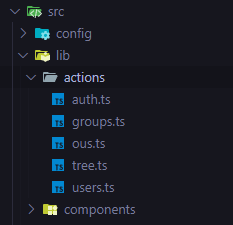
\includegraphics{images/code/bussiness-logic-modules.png}
    \caption{Módulos de la capa de logica de negocio}
    \label{fig:bussiness-logic-modules}
\end{figure}

\textbf{Principio Hollywood (Principio de Inversión de Control)}

Los módulos de alto nivel no deben depender de módulos de bajo nivel. Los módulos de bajo nivel deben depender de módulos de alto nivel. Los módulos de bajo nivel deben ser "llamados" por módulos de alto nivel y no al revés.

El diagrama de secuencia en la \autoref{fig:general-form-submission-diagram} ilustra cómo se lleva a cabo el procesamiento de una solicitud de envío de formulario en la arquitectura de n-capas del sistema, destacando la implementación del Principio de Inversión de Control (IoC).

La lógica de negocio delega la interacción con el AD al servicio de acceso a datos, siguiendo el Principio de Inversión de Control. Esto asegura que los módulos de alto nivel no dependan directamente de los módulos de bajo nivel, mejorando la flexibilidad y mantenibilidad del sistema.

\textbf{Principio Abierto-Cerrado}

El Principio Abierto-Cerrado establece que un módulo debe estar abierto para su extensión pero cerrado para su modificación. Este principio, aunque tradicionalmente asociado a la programación orientada a objetos, también es aplicable en la arquitectura de componentes en Svelte.

En lugar de modificar directamente el comportamiento de un componente, se sugiere su extensión mediante la creación de nuevos componentes o la utilización de la composición. Esto permite la introducción de nuevas funcionalidades sin alterar el código fuente original, preservando la estabilidad y confiabilidad del sistema.

Este principio se aplica en la manera en que los componentes de Svelte están diseñados para ser reutilizables y componibles. Un ejemplo claro se presenta en la \autoref{fig:open-closed-slots}, muestra cómo un mismo componente Input en Svelte puede adaptarse a través del uso de diferentes propiedades (props) y ranuras (slots), permitiendo su reutilización en distintos contextos sin necesidad de modificar su implementación base.

\begin{figure}[h]
    \centering
    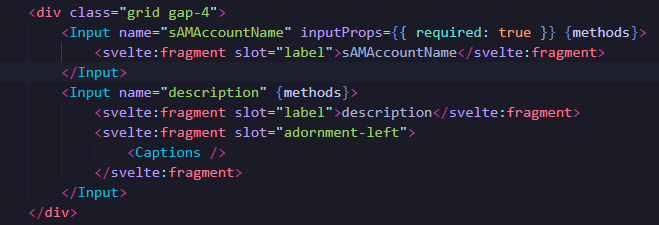
\includegraphics[width=\linewidth]{images/code/open-closed-slots.png}
    \caption{Instancias del componente Input ilustrando el pincipio Abierto-Cerrado mediante la composición de componentes}
    \label{fig:open-closed-slots}
\end{figure}